
\chapter[Delineation Of Nature]{Delineation of Nature.\\General Review of\\ Natural Phenomena}

\lettrine[lines=4]{\goudy W}{hen} the human mind first attempts to subject to its control the world of physical phenomena, and strives by meditative contemplation to penetrate the rich luxuriance of living nature, and the mingled web of free and restricted natural forces, man feels himself raised to a height from whence, as he embraces the vast horizon, individual things blend together in varied groups, and appear as if shrouded in a vapory veil. These figurative expressions are used in order to illustrate the point of view from whence we would consider the universe both in its celestial and terrestrial sphere. I am not insensible of the boldness of such an undertaking. Among all the forms of exposition to which these pages are devoted, there is none more difficult than the general delineation of nature, which we purpose sketching, since we must not allow ourselves to be overpowered by a sense of the stupendous richness and variety of the forms presented to us, but must dwell only on the consideration of masses either possessing actual magnitude, or borrowing its semblance from the associations awakened within the subjective sphere of ideas. It is by a separation and classification of phenomena, by an intuitive insight into the play of obscure forces, and by animated expressions, in which the perceptible spectacle is reflected with vivid truthfulness, that we may hope to comprehend and describe the universal all (as may) in a manner worthy of the dignity of the word Cosmos in its signification of universe, order of the world, and adornment of this universal order. May the immeasurable diversity of phenomena which crowd into the picture of nature in no way detract from that harmonious impression of rest and unity which is the ultimate object of every literary or purely artistical composition.

\begin{figure}[ht]
    %\vspace{-40pt}
    %\begin{adjustwidth}{-1cm}{-0cm}
        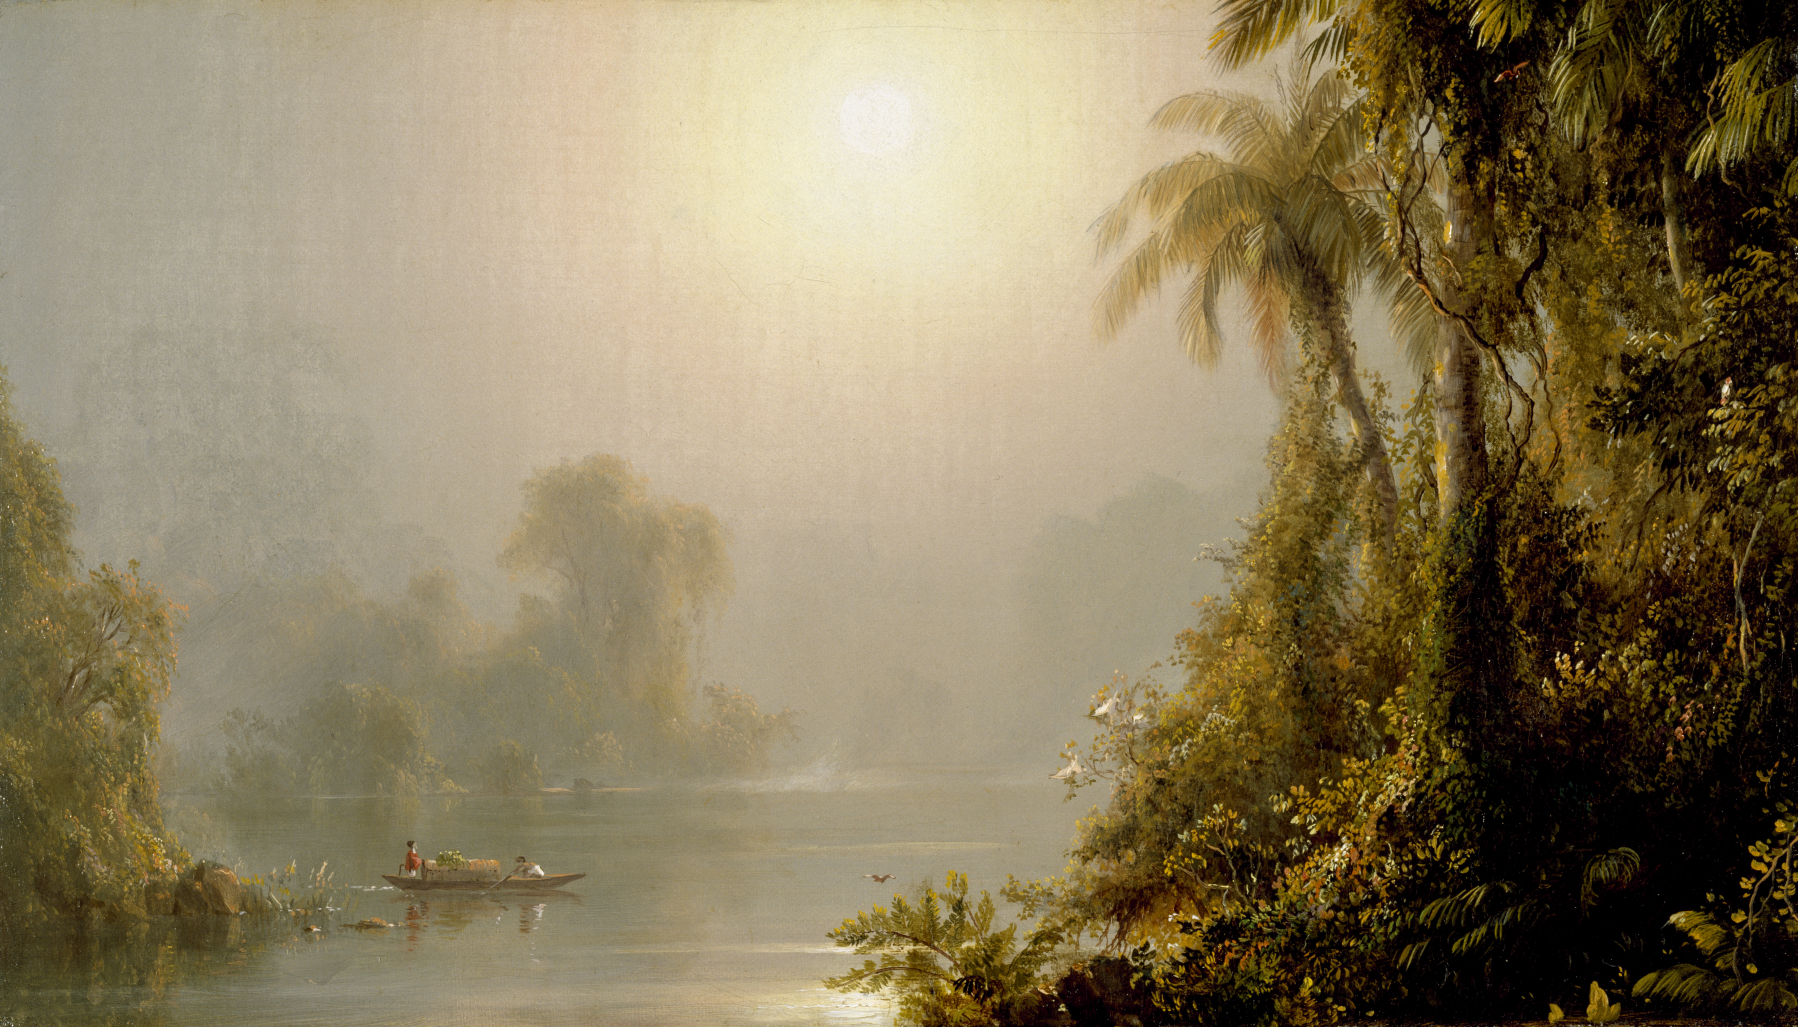
\includegraphics[width=\linewidth]{../../pictures/Frederick_Edwin_Church_-_Morning_in_the_Tropics_-_Walters_37147.jpg}
        \captionsetup{width=\linewidth}
        \caption{\footnotesize Morning in the Tropics by Frederick Edwin Church. Public domain.}
    %\end{adjustwidth}
\end{figure}

Beginning with the depths of space and the regions of remotest nebula, we will gradually descend through the starry zone to which our solar system belongs, to our own terrestrial spheroid, circled by air and ocean, there to direct our attention to its form, temperature, and magnetic tension, and to consider the fullness of organic life unfolding itself upon its surface beneath the vivifying influence of light. In this manner, a picture of the world may, with a few strokes, be made to include the realms of infinity no less than the minute microscopic animal and vegetable organisms which exist in standing waters and on the weatherbeaten surface of our rocks. All that can be perceived by the senses, and all that has been accumulated up to the present day by an attentive and variously directed study of nature, constitute the materials from which this representation is to be drawn, whose character is an evidence of its fidelity and truth. But the descriptive picture of nature which we purpose drawing must not enter too fully into detail, since a minute enumeration of all vital forms, natural objects, and processes is not requisite to the completeness of the undertaking. The delineator of nature must resist the tendency toward endless division, in order to avoid the dangers presented by the very abundance of our empirical knowledge. A considerable portion of the qualitative properties of matter or, to speak more in accordance with the language of natural philosophy, of the qualitative expression of forces is doubtlessly still unknown to us, and the attempt perfectly to represent unity in diversity must therefore necessarily prove unsuccessful. Thus, besides the pleasure derived from acquired knowledge, there lurks in the mind of man; and tinged with a shade of sadness, an unsatisfied longing for something beyond the present, a striving toward regions yet unknown and unopened. Such a sense of longing binds still faster the links which, in accordance with the supreme laws of our being, connect the material with the ideal world, and animates the mysterious relation existing between that which the mind receives from without, and that which it reflects from its own depths to the external world. If, then, nature (understanding by the term all natural objects and phenomena) be illimitable in extent and contents, it likewise presents itself to the human intellect as a problem which can not be grasped, and whose solution is impossible, since it requires a knowledge of the combined action of all natural forces. Such an acknowledgment is due where the actual state and prospective development of phenomena constitute the sole objects of direct investigation, which does not venture to depart from the strict rules of induction. But, although the incessant effort to embrace nature in its universality may remain unsatisfied, the history of the contemplation of the universe (which will be considered in another part of this work) will teach us how, in the course of ages, mankind has gradually attained to a partial insight into the relative dependence of phenomena. My duty is to depict the results of our knowledge in all their bearings with reference to the present. In all that is subject to motion and change in space, the ultimate aim, the very expression of physical laws, depend upon mean numerical values, which show us the constant amid change, and the stable amid apparent fluctuations of phenomena. Thus the progress of modern physical science is especially characterized by the attainment and the rectification of the mean values of certain quantities by means of the processes of weighing and measuring; and it may be said, that the only remaining and widely diffused hieroglyphic characters still in our writing numbers appear to us again, as powers of the Cosmos, although in a wider sense than that applied to them by the Italian School.

The earnest investigator delights in the simplicity of numerical relations, indicating the dimensions of the celestial regions, the magnitudes and periodical disturbances of the heavenly bodies, the triple elements of terrestrial magnetism, the mean pressure of the atmosphere, and the quantity of heat which the sun imparts in each year, and in every season of the year, to all points of the solid and liquid surface of our planet. These sources of enjoyment do not, however, satisfy the poet of Nature, or the mind of the inquiring many. To both of these, the present state of science appears as a blank, now that she answers doubtingly, or wholly rejects as unanswerable, questions to which former ages deemed they could furnish satisfactory replies. In her severer aspect, and clothed with less luxuriance, she shows herself deprived of that seductive charm with which a dogmatizing and symbolizing physical philosophy knew how to deceive the understanding and give the rein to imagination. Long before the discovery of the New World, it was believed that new lands in the Far West might be seen from the shores of the Canaries and the Azores. These illusive images were owing, not to any extraordinary refraction of the rays of light, but produced by an eager longing for the distant and the unattained. The philosophy of the Greeks, the physical views of the Middle Ages, and even those of a more recent period, have been eminently imbued with the charm springing from similar illusive phantoms of the imagination. At the limits of circumscribed knowledge, as from some lofty island shore, the eye delights to penetrate to distant regions. The belief in the uncommon and the wonderful lends a definite outline to every manifestation of ideal creation; and the realm of fancy -- a fairyland of cosmological, geognostical, and magnetic visions -- becomes thus involuntarily blended with the domain of reality.

Nature, in the manifold signification of the word -- whether considered as the universality of all that is and ever will be, as the inner moving force of all phenomena, or as their mysterious prototype -- reveals itself to the simple mind and feelings of man as something earthly and closely allied to himself. It is only within the animated circles of organic structure that we feel ourselves peculiarly at home. Thus, wherever the earth unfolds her fruits and flowers and gives food to countless tribes of animals, there the image of nature impresses itself most vividly upon our senses. The impression thus produced upon our minds limits itself almost exclusively to the reflection of the earthly. The starry vault and the wide expanse of the heavens belong to a picture of the universe in which the magnitude of masses, the number of congregated suns and faintly glimmering nebulae, although they excite our wonder and astonishment, manifest themselves to us in apparent isolation and as utterly devoid of all evidence of their being the scenes of organic life. Thus, even in the earliest physical views of mankind, heaven and earth have been separated and opposed to one another as an upper and lower portion of space. If, then, a picture of nature were to correspond to the requirements of contemplation by the senses, it ought to begin with a delineation of our native earth. It should depict, first, the terrestrial planet as to its size and form; its increasing density and heat at increasing depths in its superimposed solid and liquid strata; the separation of sea and land, and the vital forms animating both, developed in the cellular tissues of plants and animals; the atmospheric ocean, with its waves and currents, through which pierce the forest-crowned summits of our mountain chains. After this delineation of purely telluric relations, the eye would rise to the celestial regions, and the Earth would then, as the well-known seat of organic development, be considered as a planet, occupying a place in the series of those heavenly bodies which circle round one of the innumerable host of self-luminous stars. This succession of ideas indicates the course pursued in the earliest stages of perceptive contemplation and reminds us of the ancient conception of the sea-girt disk of earth, supporting the vault of heaven. It begins to exercise its action at the spot where it originated, and passes from the consideration of the known to the unknown, of the near to the distantIt corresponds with the method pursued in our elementaryworks on astronomy (and which is so admirable in a mathematical point of view), of proceeding from the apparent to thereal movements of the heavenly bodies.
